\section{Anwendungsarchitektur}
\label{app_architecture}
Dieser Abschnitt beschreibt das implementierte System in der Gesamtheit. Das zu implementierende Werkzeug kann in zwei Bereiche gegliedert werden, dem Android-Client und dem HTTP-Server. 
Grundlegend handelt es sich hier um eine klassische Client-Server Architektur, bei der verschiedenartige Clients zum Einsatz kommen.

Der Server basiert auf Node.js.

Dadurch wird eine Abstraktion vom Betriebssystem erreicht.
Die zugrunde liegende Datenbank für die Persistenz ist MySQL, welches für verschiedene Plattformen verfügbar ist.
Für die Videokonvertierung wird AVLib benutzt, auch diese Software ist für verschiedene Plattformen verfügbar. Details zu den Serverkomponenten sind in Abschnitt \ref{server} zu finden.

Als Clients kommen einerseits die entwickelte Android-Bibliothek zum Einsatz, als auch handelsübliche Webbrowser.

Die einzelnen Komponenten und die Kommunikationsbeziehungen sind in Abbildung \ref{fig:architecture} dargestellt.

\begin{figure}[htb]
	\centering
	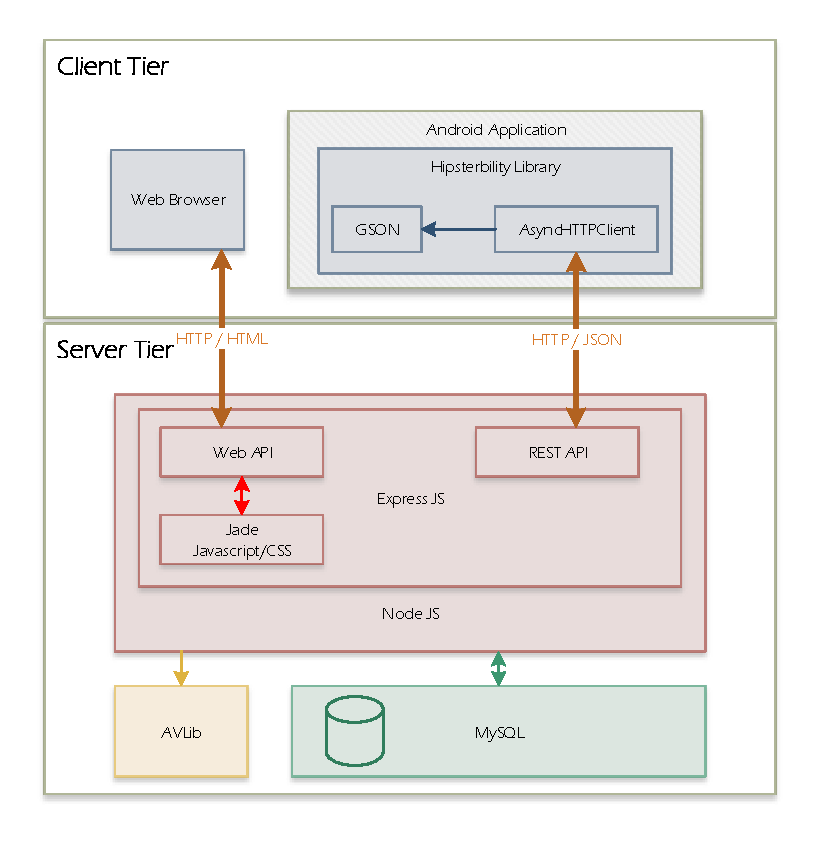
\includegraphics[width=0.75\linewidth]{img/architecture}
	\caption{hipsterbility Framework Architektur\label{fig:architecture}}
\end{figure}

\subsection{Client-Server-Kommunikation}
Nachfolgend werden die einzelnen Architekturkomponenten kurz betrachtet und in das Gesamtbild eingefügt. Hier liegt der Fokus auf der allgemeinen Kommunikationsbeziehung zwischen den einzelnen Elementen.


\subsubsection{Server}
Wie bereits erwähnt basiert der Server auf Node JS und nutzt Express JS als Webserver.
Dieser bietet zwei \ac{API}s an, eine Web API für Webbrowser und eine REST API für die reine Datenübertragung.

Die Kommunikation mit der MySQL Datenbank erfolgt über einen entsprechenden Datenbank Treiber.
Auch für AVLib existiert ein entsprechender Wrapper, welcher die Nutzung erleichtert.
Details zum Aufbau des Servers sind in Abschnitt \ref{server} zu finden.


\subsubsection{Webbrowser-Client}
Die Kommunikationsstruktur ist für den Webbrowser Client als reiner Online-Dienst ausgelegt.
Dies bedeutet, dass der Client die -- vom Server abgerufenen -- Daten nicht dauerhaft zwischenspeichern, sondern nur zur Darstellung und für die aktuelle Funktionserfüllung nutzen.
Für die abgerufenen Daten erfüllen der Browser nur die Funktion des \emph{Renderers}, da die Aufbereitung bereits vom Server vorgenommen wird.

Übertragen werden fertige HTML-Seiten mit Javascript und \ac{CSS}.
Diese werden mit \emph{Jade}-Skripten erstellt (siehe Abschnitt \ref{sec:node-mudules}) und über die Web API des Webservers ausgeliefert.
Eine ausführliche Erläuterung des webbasierten Verwaltungstools \ref{sec:web_verwaltung}.


\subsubsection{Android-Client}
Bei der Android Bibliothek handelt es sich um eine Hybrid-Online Lösung.
Zu Beginn werden Daten vom Server abgerufen, nach der initialen Kommunikation speichert der Client Daten zwischen, die erst am Ende der Ausführung an den Server übertragen werden.
Zwischen diesen beiden Kommunikationsbeziehungen benötigt der Client keine dauerhafte Serververbindung.

Der Android-Client kann seine Funktion jedoch nicht ohne Serververbindung aufnehmen, diese wird an zwei Zeitpunkten, wie beschrieben, zwingend benötigt.
Der Datenaustausch zwischen Client und Server erfolgt über eine REST API, welche in Abschnitt \ref{sec: api} genauer beschrieben wird.

Die Daten werden in der \ac{JSON} Notation im HTML-Body vom Server abgerufen, bzw. als MultiPart Daten über HTTP vom Client zum Server übertragen.
Eine detaillierte Beschreibung des Android-Clients erfolgt in Abschnitt \ref{sec:android_client}.